%************AUSWERTUNG****************
\section{Evaluation}
\label{sec:evaluation}

For evaluation purposes, the scripting language \verb|Python| \cite{PYTHON} is utilized.
The Python libraries, \verb|numpy| \cite{harris2020array}, \verb|pandas| \cite{reback2020pandas}, \verb|scipy| \cite{2020SciPy-NMeth} and \verb|matplotlib| \cite{Hunter:2007} are used for statistical calculation operations, reading and processing data and creating plots.

Unless specified otherwise, the maximum uncertainty method according to Equation \ref{equ:groestunsicherheit} \cite{MMETH} is used for all uncertainty calculations.
For this purpose, the total differential of the outgoing equation is formed and the absolute values of the summands are multiplied by the uncertainty determined.
Statistical evaluations are subject to a statistical uncertainty according to the Student-t distribution.
\begin{equation}
    \varDelta f = \biggl| \frac{\partial f}{\partial x_{1}} \cdot \varDelta x_{1} \biggl| + \biggl| \frac{\partial f}{\partial x_{2}} \cdot \varDelta x_{2} \biggl| + .... + \biggl| \frac{\partial f}{\partial x_{n}} \cdot \varDelta x_{n} \biggl|
    \label{equ:groestunsicherheit}
\end{equation}

In the present evaluation, the library \verb|uncertainties| \cite{UN} is used for calculating any uncertainty propagation, as this is based on the principle of the maximum uncertainty method as described in Equation \ref{equ:groestunsicherheit}.

\subsection{Laser Source Characterization}
In order to obtain the central wavelenght and the full width half maximum $FWHM$, the data in Table \ref{tab:execution:infrared-characterization} is fitted using the function \verb|curve_fit|.
The measured IR spectra is fitted using a sum of multiple gaussian distributions,as seen in Equation \ref{eq:evaluation:fitfunc}.
For convinience the spectra was devided by the maximum value of the emission lines. 

\begin{equation}
    G_{comb}(\lambda) = \sum_{p = 1} A_p e^{-\frac{(\lambda - \lambda_p)^{2}}{2 \sigma_{p}^2}}  = \sum_{p = 1} G_p(\lambda)
    \label{eq:evaluation:fitfunc}
\end{equation}
Judging by the estimated parameters in Table \ref{tab:evaluation:ir_fitted1} , the emission spectrum of Ytterbium reduces to 7 indiviuall lines resulting in a bimodal structure.
The resulting function is then normalized by integrating and over the defined space to get a power density.
Using Equation \ref{eq:evaluation:central} the central wavelenght $\langle \lambda \rangle$ is calculated by integrating over $\lambda G_{comb}(\lambda)$, where $G_{comp}$ is the superposition of gauss distributions. 
\begin{equation}
    \langle \lambda \rangle = \frac{1}{K} \int_{P}\lambda G_{comp}(\lambda) d \lambda
    \label{eq:evaluation:central}
\end{equation}
\monofig{width=\textwidth}{IR_fitted.pdf}{
    Emission spectra of Yb Laser and its fit function. \\
    $G_i(\lambda_p)$ = Gaussian fitfunctions with corresponding wavelengths $\lambda_p$ at peakpositions,
    $G_{comb}(\lambda)$ = Superposition of all gaussian fitfunctions,
    $\lambda_c$ = central wavelength,
    $FWHM_{total}$ = total full width half maximum
     }{fig:evaluation:ir_fitted}
The outer most peaks are used to estimate the FWHM by using the the relation $FWHM = 2 \sqrt{2 \ln(2)} \cdot \sigma$ which holds for all gauss distribution.
Now the distance between the two outermost FWHM points is calculate to estimate the total full width half maximum $FWHM_{total}$ as seen in Figure \ref{fig:evaluation:ir_fitted}.
The error estimates for the fitfunction were calculated using the diagonal elements of the covariance matrix obtained by the library routine, which are an estimation for the variance of the fitparameters.
Further discussion regarding the results are in Section \ref{sec:discussion}.
\begin{table}[H]
\centering
\caption{
    Fitting Parameter Laser Source Characterization. \\
    $A_p$: Gaussian Amplitudes,
    $\lambda_p$: Expectation value,
    $\sigma_p$: Standart diviations,
    $G_p$: functions associated with the parameters,
}
\begin{tabular}{c|ccc} \hline
    &  $A_p$ / 1 &  $\lambda_p$ / nm & $\sigma_p$ \\ \hline  \hline 
$G_0$&$0.40 \pm 0.07$&$1012.37 \pm 0.04$&$1.03 \pm 0.05$\\ \hline
$G_1$&$0.63 \pm 0.13$&$1014.46 \pm 0.13$&$1.71 \pm 0.18$\\ \hline
$G_2$&$0.445 \pm 0.014$&$1025.25 \pm 0.26$&$5.52 \pm 0.41$\\ \hline
$G_3$&$0.46 \pm 0.08$&$1017.63 \pm 0.51$&$2.80 \pm 0.34$\\ \hline
$G_4$&$0.490 \pm 0.009$&$1038.46 \pm 0.24$&$5.89 \pm 0.22$\\ \hline
$G_5$&$0.43 \pm 0.04$&$1046.49 \pm 0.31$&$2.70 \pm 0.19$\\ \hline
$G_6$&$0.57 \pm 0.06$&$1049.50 \pm 0.03$&$1.69 \pm 0.05$\\ \hline
\end{tabular}
\label{tab:evaluation:ir_fitted1}
\end{table}
\newpage
\subsection{SHG Characterization}
Using the same methods as before, a fitting function is estimated and afterwards the central wavelenght $\langle \lambda \rangle$.
The spectrum is devided by the maximum Intensity.
As the inviduall peaks are quite good resolved, it would not make sence to estimate the FWHM and therefore only the individual FWHM are calculated.
While two of the peaks in the SHG Spectrum doesnt show up in the residual IR Spectrum, other maxima including the central wavelength align nicely with SHG predictions.

\duofigcom{SHG_fitteddx1.pdf}{fig:evaluation:greenfitted}{SHG_fitteddx2.pdf}{fig:evaluation:redfitted}{
    (a) Second Harmonic Generation spectrum. (b) Residuel Spectrum \\
    $G_i(\lambda_p)$ = Gaussian fitfunctions with corresponding wavelengths $\lambda_p$ at peakpositions,
    $G_{comb}(\lambda)$ = Superposition of all gaussian fitfunctions,
    $\lambda_c$ = central wavelength,
    }
    {fig:evaluation:shg_fitted}
The residual IR Spectrum has substantially more noice than the other spectra, because its maximal intensity is so low.
This results in less precise fitting and a long parameter convergence time.
To get the conversionrate $C$ first the fitting function of the SHG spectrum is integrated over the relevant intervall around the peaks. 
Then it is devided by the sum of the two fitting functions in Figure \ref{fig:evaluation:shg_fitted} and integrated.:
\begin{align}
    C &= \frac{\int_{\varOmega} G_{SHG}(\lambda) d \lambda}{ \int_{\Sigma} (G_{SHG}(\lambda) + G_{IR}(\lambda))d \lambda} \\
    C &= 0.84 \pm 0.02 
\end{align}

\begin{table}[H]
    \label{}
    \centering
    \caption{Fitting Parameter SHG Spectrum. \\
    $A_p$: Gaussian Amplitudes,
    $\lambda_p$: Expectation value,
    $\sigma_p$: Standart diviations,
    $G_p$: functions associated with the parameters,}
    
    \begin{tabular}{c|ccc} \hline
        &  $A_p$ / 1 &  $\lambda_p$ / nm & $\sigma_p$ \\ \hline \hline 
    $G_0$&$0.27 \pm 0.03$&$509.25 \pm 0.22$&$1.48 \pm 0.09$\\ \hline
    $G_1$&$0.61 \pm 0.10$&$510.96 \pm 0.14$&$0.83 \pm 0.09$\\ \hline
    $G_2$&$0.54 \pm 0.14$&$511.92 \pm 0.04$&$0.57 \pm 0.03$\\ \hline
    $G_3$&$0.49 \pm 0.01$&$514.38 \pm 0.01$&$0.46 \pm 0.01$\\ \hline
    $G_4$&$0.11 \pm 0.01$&$517.99 \pm 0.03$&$0.79 \pm 0.03$\\ \hline
    $G_5$&$0.14 \pm 0.05$&$521.50 \pm 0.04$&$0.83 \pm 0.10$\\ \hline
    $G_6$&$0.11 \pm 0.03$&$522.81 \pm 0.65$&$1.34 \pm 0.21$\\ \hline
    \end{tabular}
    \end{table}

\begin{table}[H]
        \label{}
        \centering
        \caption{Fitting Parameter Residual Spectrum. \\
        $A_p$: Gaussian Amplitudes,
        $\lambda_p$: Expectation value,
        $\sigma_p$: Standart diviations,
        $G_p$: functions associated with the parameters,}
        \begin{tabular}{c|ccc} \hline
            &  $A_p$ / 1 &  $\lambda_p$ / nm & $\sigma_p$ \\ \hline  \hline 
        $G_0$&$0.83 \pm 0.03$&$1015.73 \pm 0.16$&$2.75 \pm 0.09$\\ \hline
        $G_1$&$0.57 \pm 0.03$&$1021.50 \pm 0.21$&$2.56 \pm 0.13$\\ \hline
        $G_2$&$0.10 \pm 0.02$&$1028.65 \pm 0.14$&$0.82 \pm 0.15$\\ \hline
        $G_3$&$0.38 \pm 0.17$&$1035.31 \pm 0.41$&$3.12 \pm 0.44$\\ \hline
        $G_4$&$0.58 \pm 0.09$&$1040.73 \pm 1.21$&$4.61 \pm 0.54$\\ \hline
        \end{tabular}
\end{table}   
    
\subsection{Iodine Absorbance}
\label{sec:evaluation:iodine-absorbance}

Given the transmitted intensities documented in tables \ref{tab:execution:iodine:single:1} to \ref{tab:execution:iodine:triple}, they can be plotted as a function of the respective wavelengths $\lambda$ as shown in Figure \ref{fig:evaluation:transmission}.

Using Equation \ref{eq:fundamentals:absorbance}, the absorbance $A$ can be calculated from the obtained transmission spectra. For the different configurations, the resulting absorbance $A$ as a function of the wavelength $\lambda$ is shown in figures \ref{fig:evaluation:absorbance:single:1} to \ref{fig:evaluation:absorbance:triple}. In order to make absorption more visible, a Savitzky–Golay filter using \verb|scipy.signal.savgol_filter| with a window length of $15$ and polynomial order of $1$ are applied to the plotted absorbance. Furthermore, in order to make it easier to identify expected absorption peaks in the recorded absorbance the molar absorption coefficient $\varepsilon$ - which is used later for calculating the concentration $c$ of iodine - is plotted on a second axis.

Using Equation \ref{eq:fundamentals:absorptivity}, the absorption coefficient $\varepsilon$ is obtained from the absorption cross-section $\sigma$ taken from related literature \cite{Iodine}. In the area of $\lambda = \SI{508}{\nm}$ to $\lambda = \SI{511}{\nm}$ orange vertical lines relate the peaks of the measured absorbance $A$ to the peaks of the literature spectrum.

\begin{figure}[H]
    \centering
    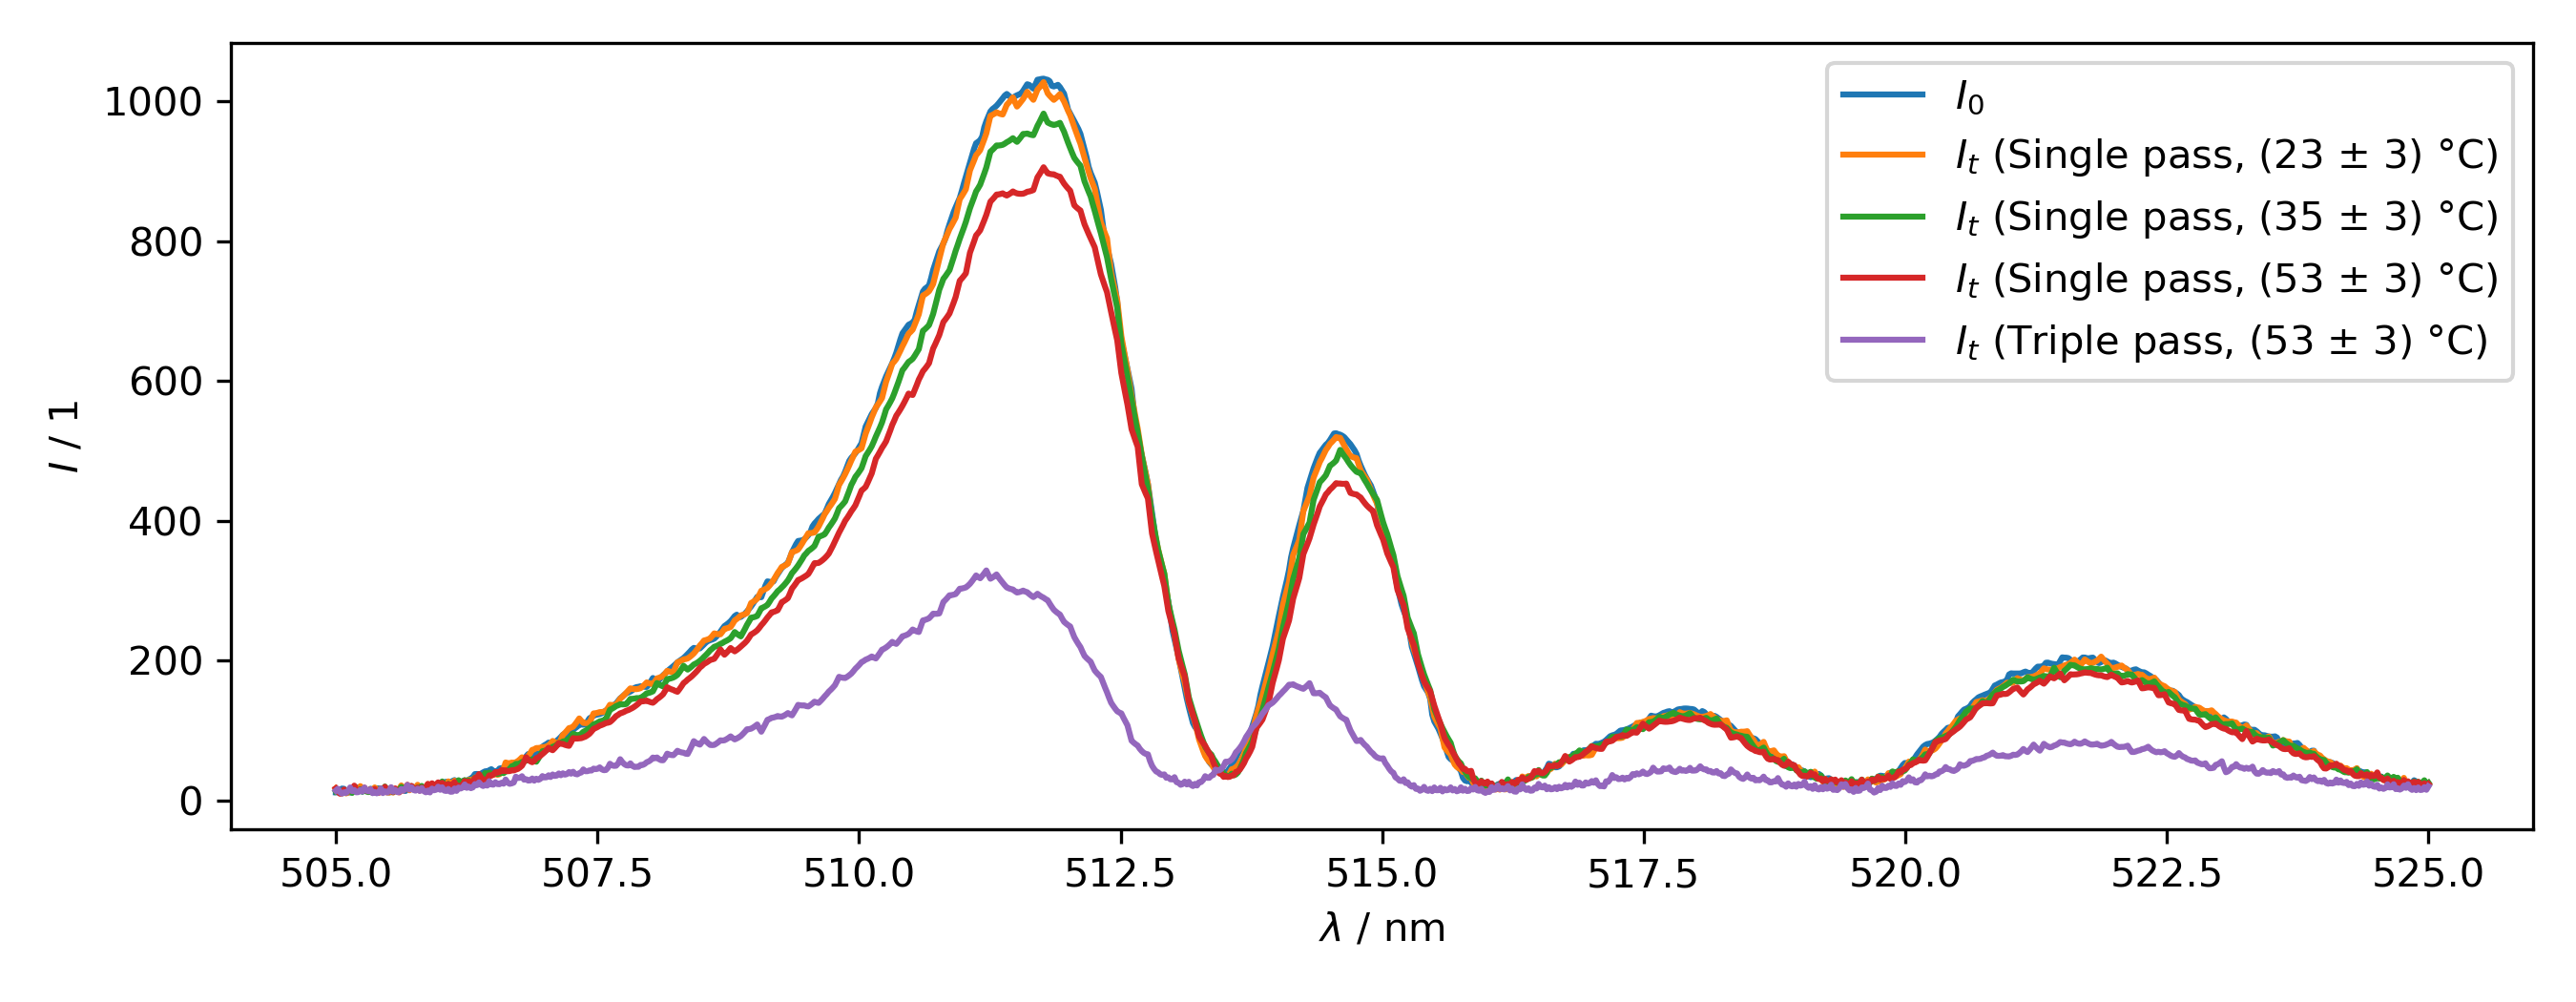
\includegraphics[width=\textwidth]{graphics/transmission.png}
    \caption{Transmission spectra without iodine as well as for single-pass and triple-pass configurations.\\
        $I_0$ = Intensity without iodine, $I_t$ = Intensity transmitted through iodine}
    \label{fig:evaluation:transmission}
\end{figure}

\begin{figure}[H]
    \centering
    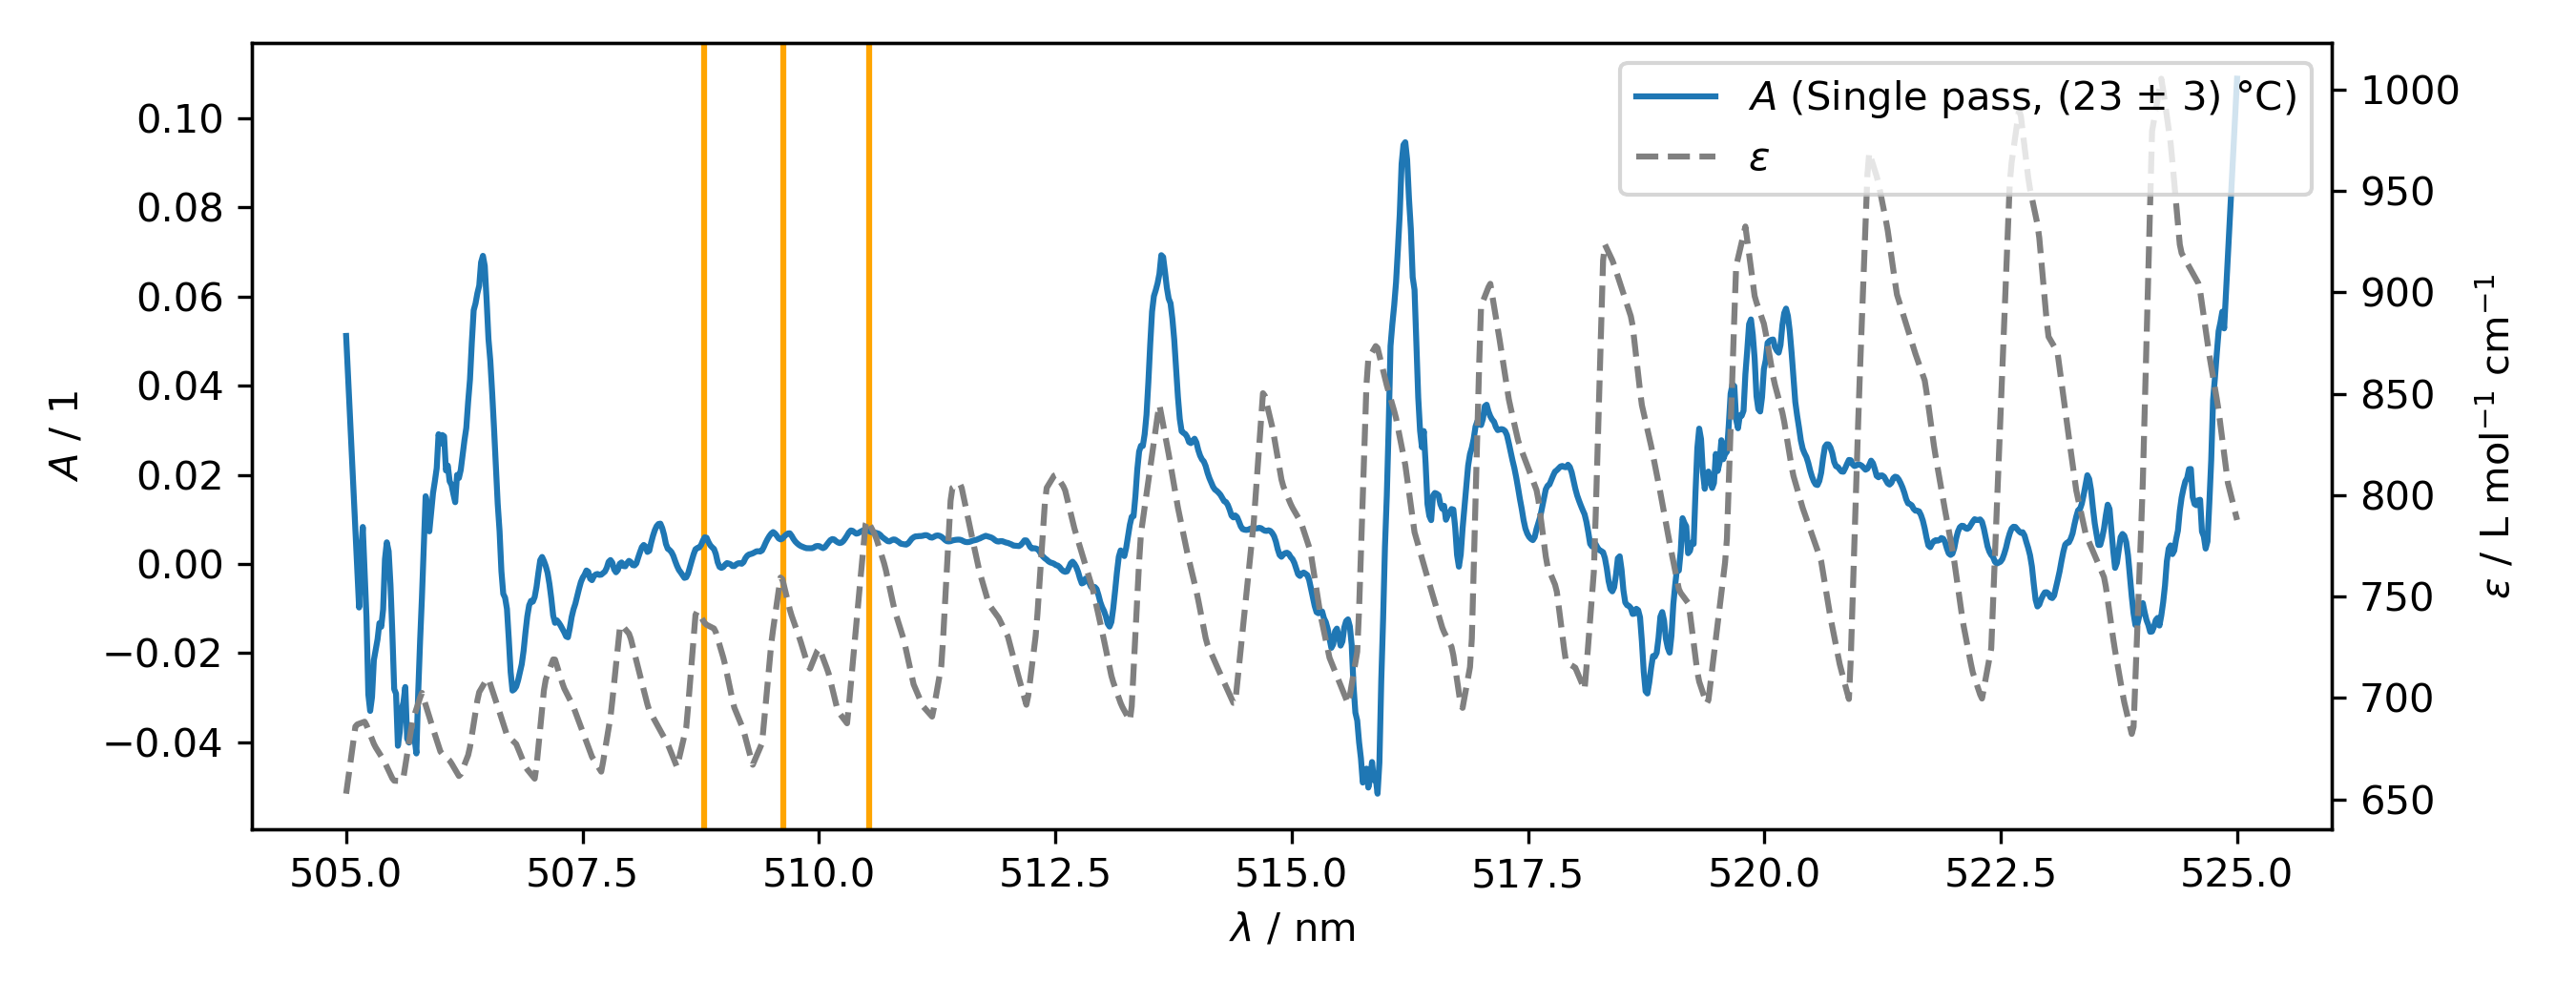
\includegraphics[width=\textwidth]{graphics/absorbance-25.png}
    \caption{Absorbance and used molar absorption coefficient as functions of wavelength.\\
        $A$ = Absorbance, $\varepsilon$ = Molar absorption coefficient, $\lambda$ = Wavelength}
    \label{fig:evaluation:absorbance:single:1}
\end{figure}

\begin{figure}[H]
    \centering
    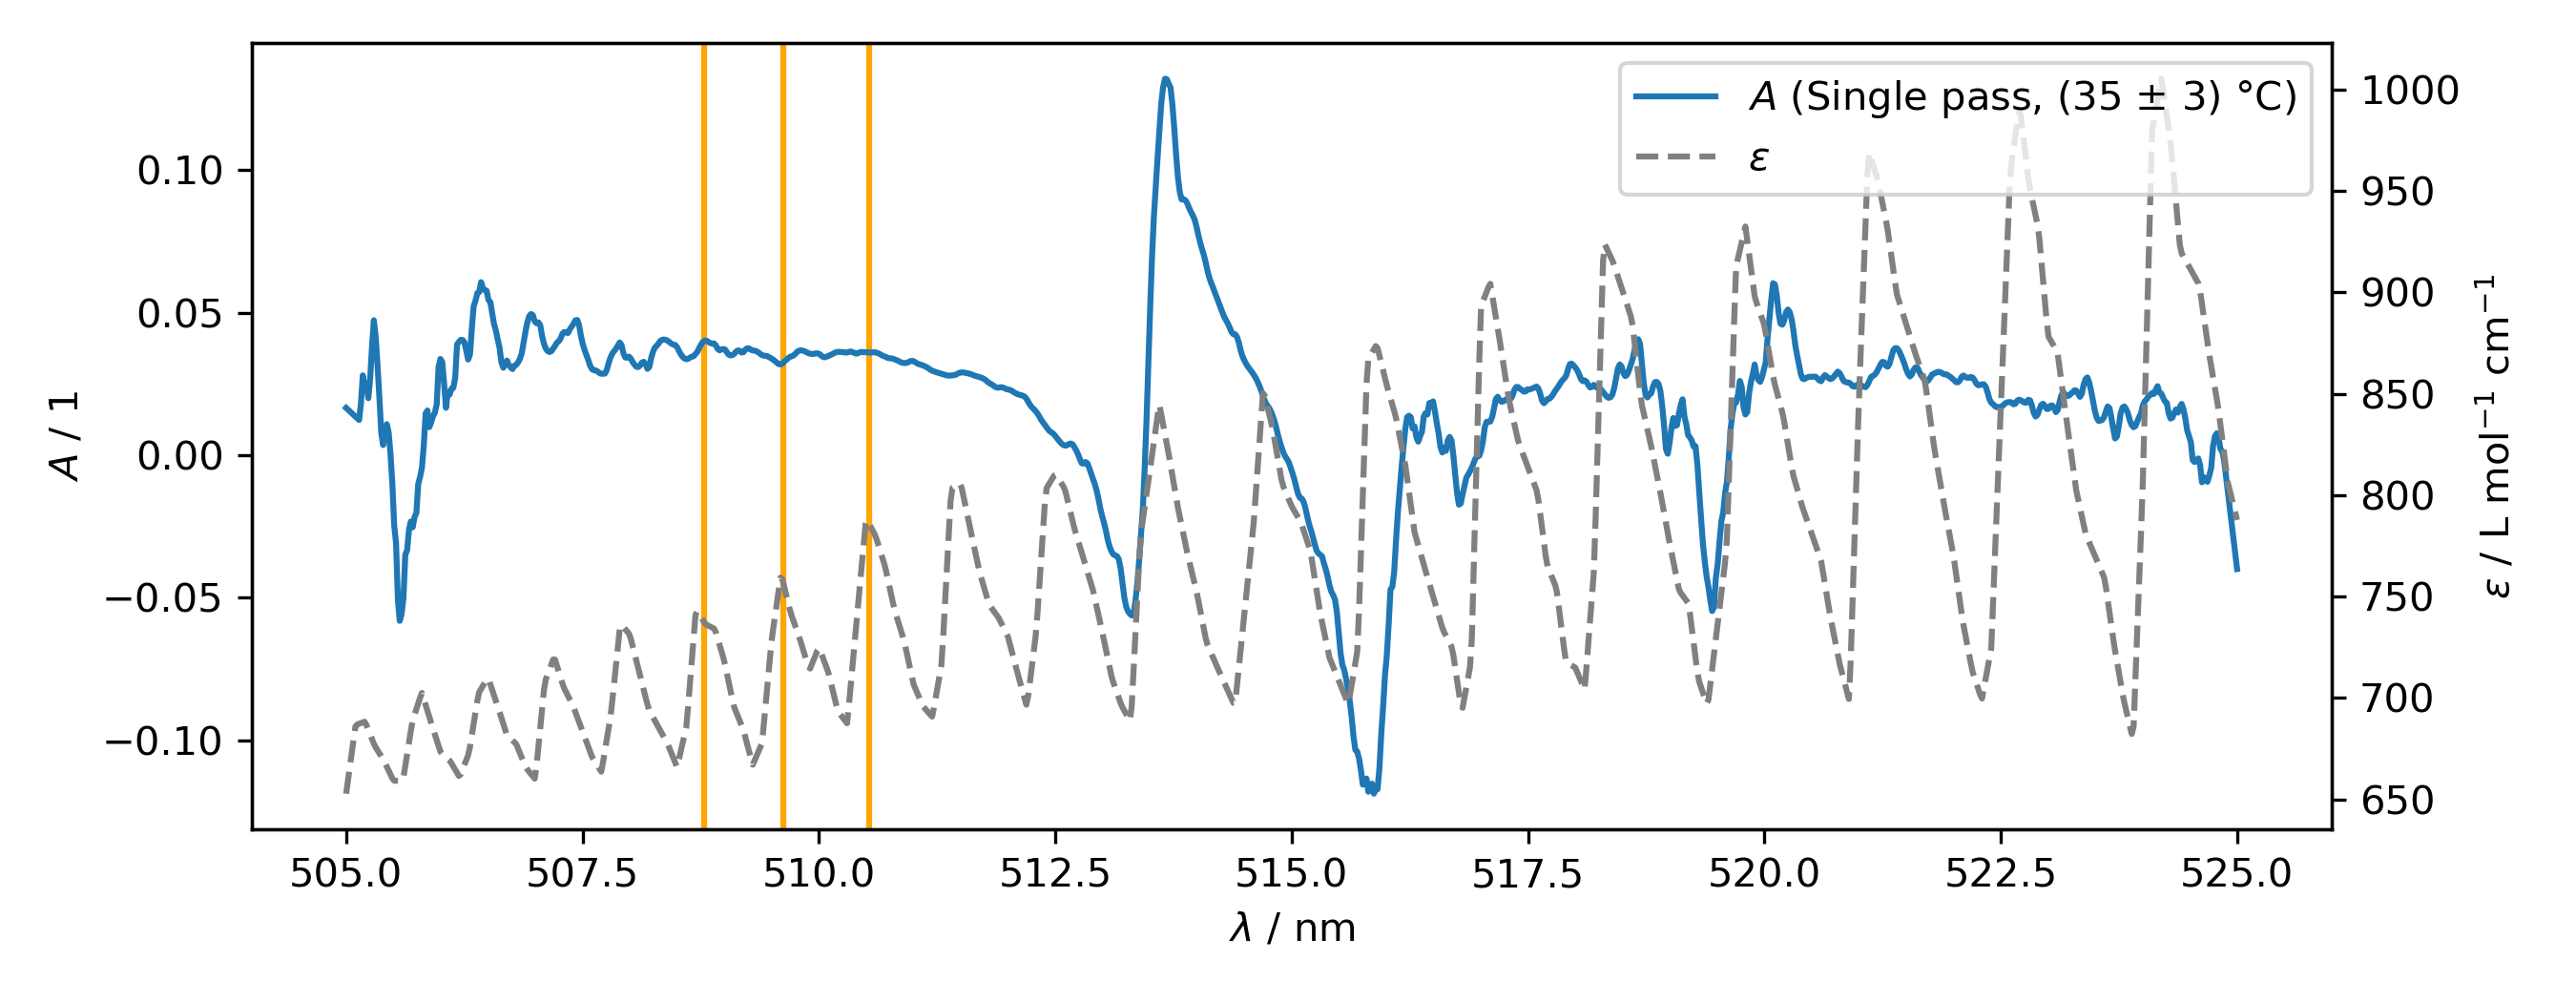
\includegraphics[width=\textwidth]{graphics/absorbance-42.png}
    \caption{Absorbance and used molar absorption coefficient as functions of wavelength.\\
        $A$ = Absorbance, $\varepsilon$ = Molar absorption coefficient, $\lambda$ = Wavelength}
    \label{fig:evaluation:absorbance:single:2}
\end{figure}

\begin{figure}[H]
    \centering
    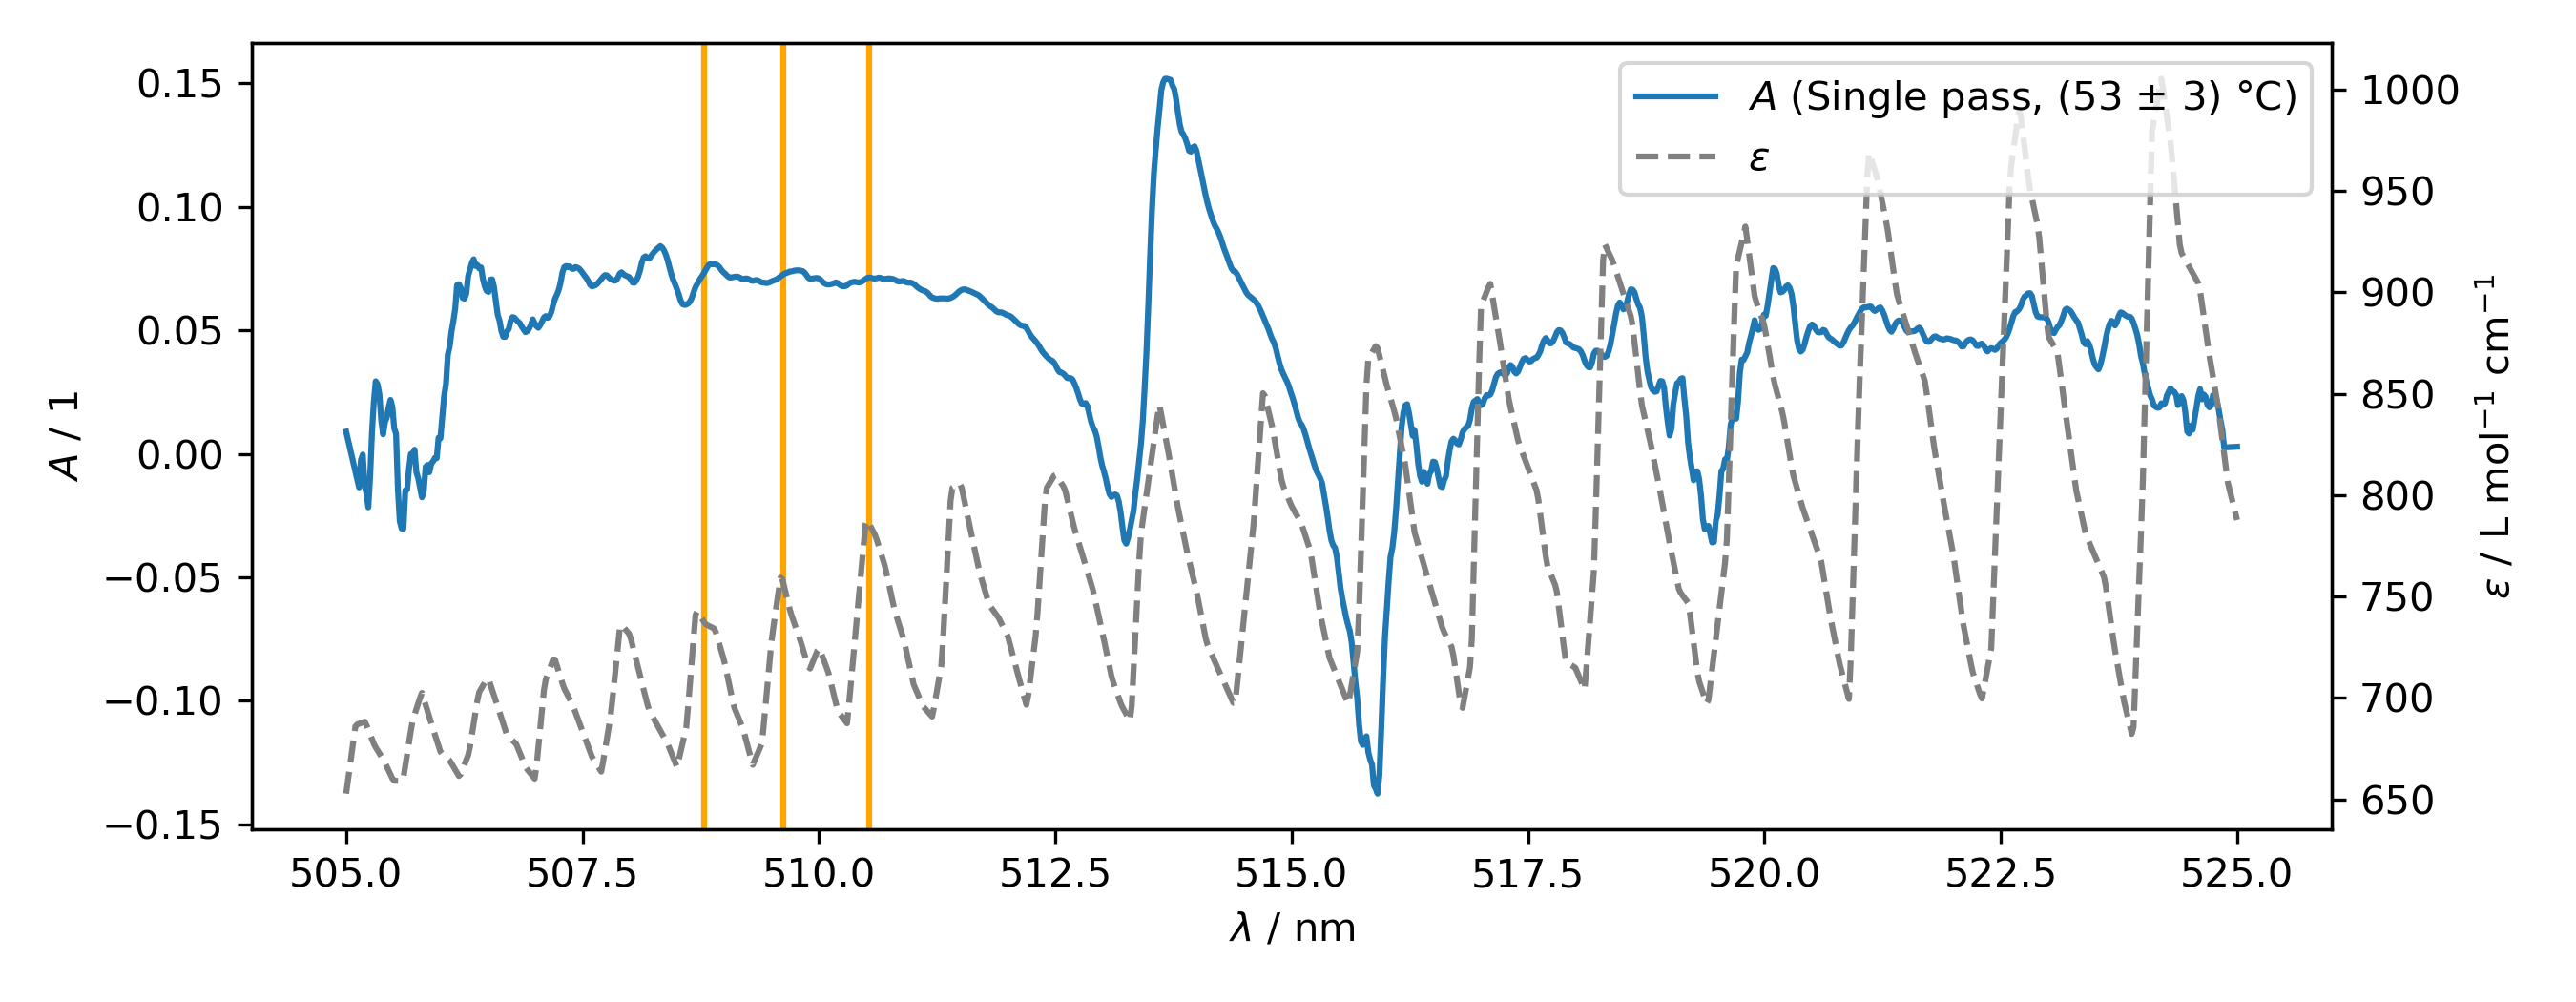
\includegraphics[width=\textwidth]{graphics/absorbance-60.png}
    \caption{Absorbance and used molar absorption coefficient as functions of wavelength.\\
        $A$ = Absorbance, $\varepsilon$ = Molar absorption coefficient, $\lambda$ = Wavelength}
    \label{fig:evaluation:absorbance:single:3}
\end{figure}

\begin{figure}[H]
    \centering
    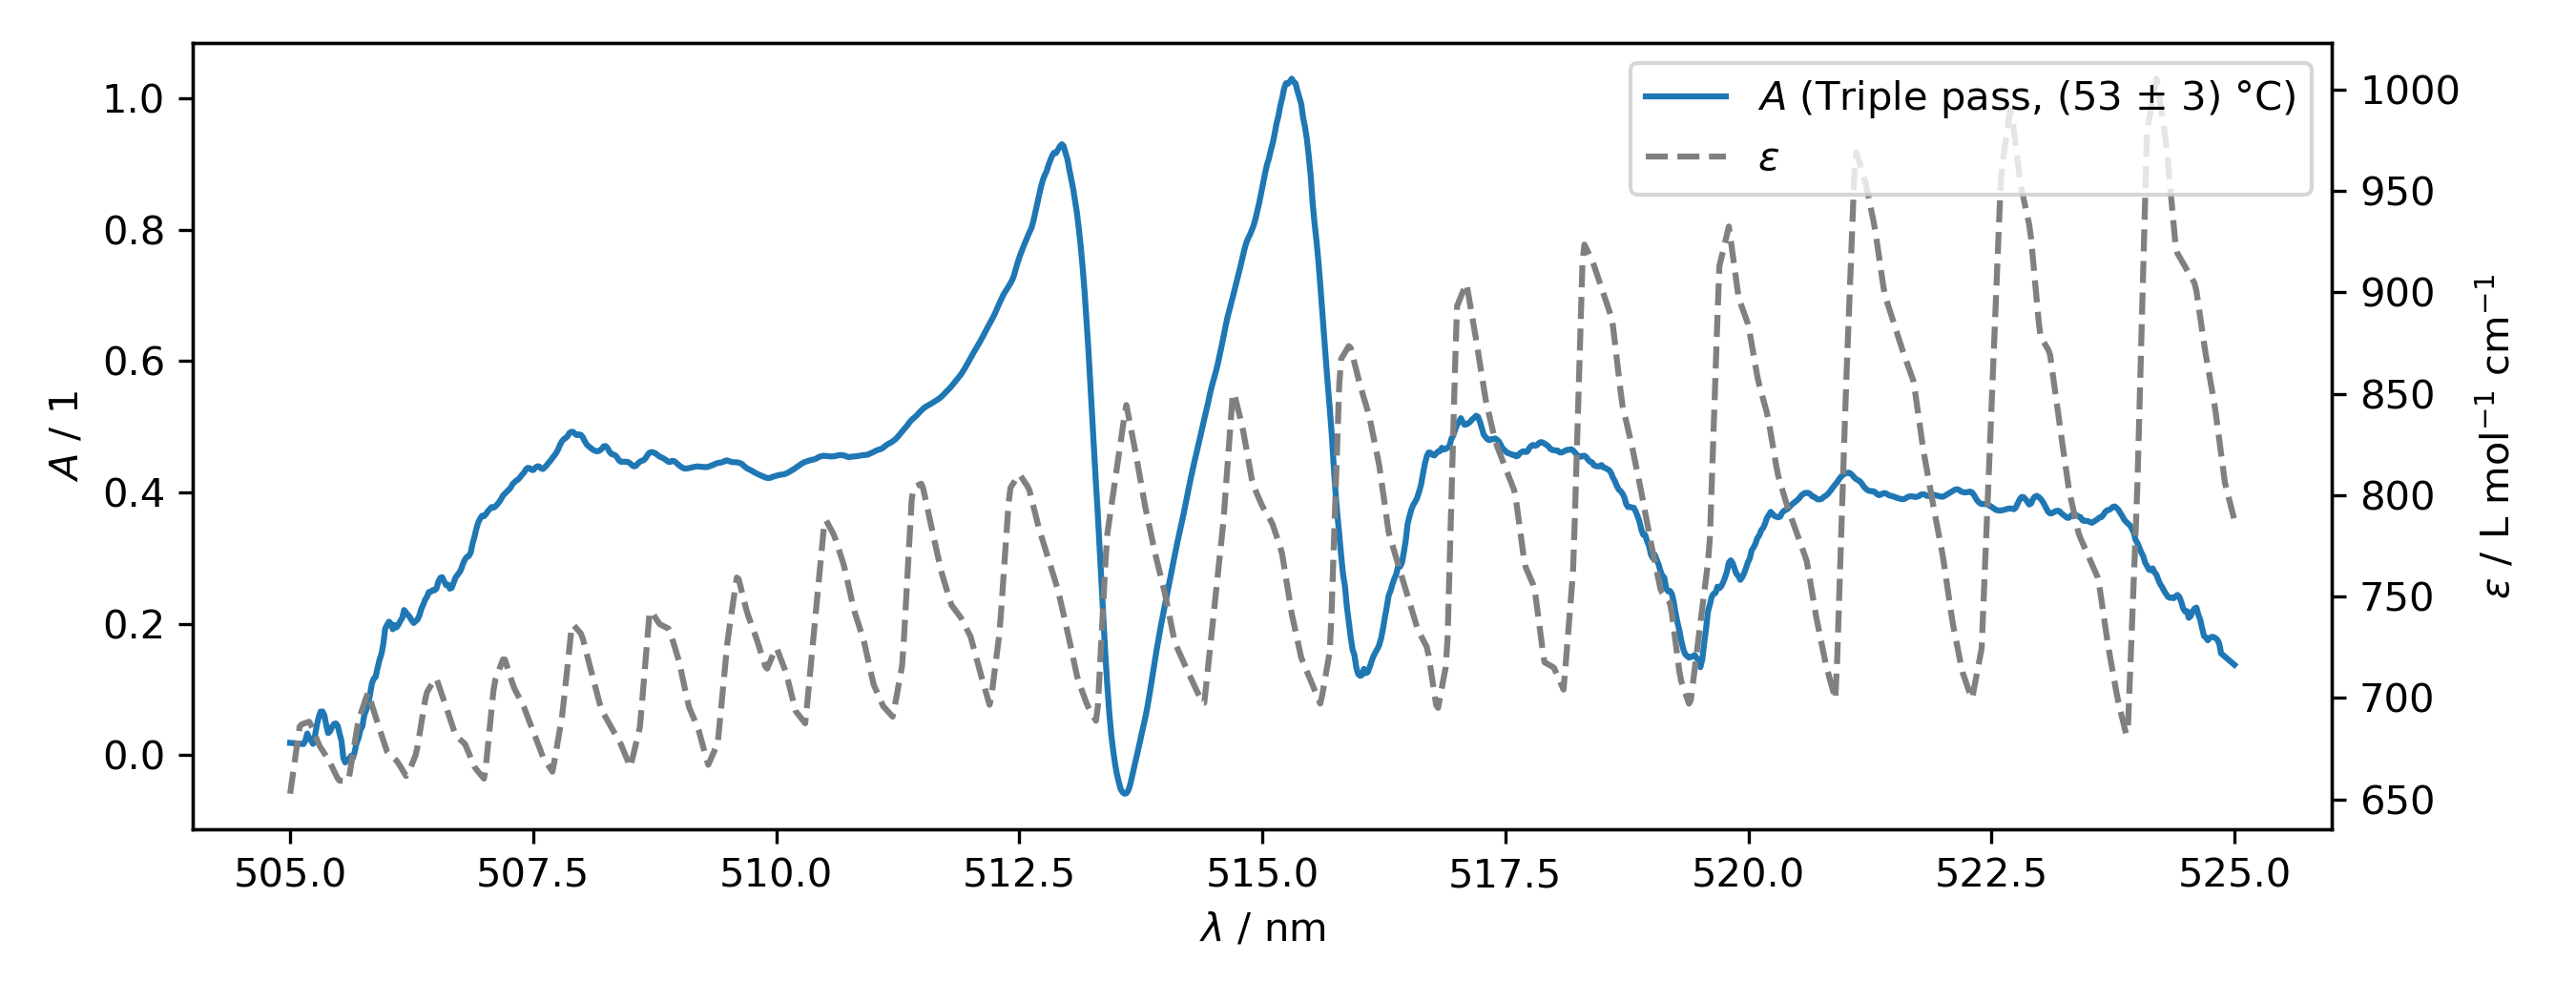
\includegraphics[width=\textwidth]{graphics/absorbance-triple.png}
    \caption{Absorbance and used molar absorption coefficient as functions of wavelength.\\
        $A$ = Absorbance, $\varepsilon$ = Molar absorption coefficient, $\lambda$ = Wavelength}
    \label{fig:evaluation:absorbance:triple}
\end{figure}

\subsection{Iodine Concentration}
\label{sec:evaluation:iodine-concentration}

Using Equation \ref{eq:fundamentals:beer} as well as the absorbance $A$ and molar absorption coefficient $\varepsilon$ obtained in Section \ref{sec:evaluation:iodine-absorbance}, the concentration $c$ of molecular iodine in the cell can be calculated.
For this, the effective path-length $l$ of the laser beam passing through gaseous iodine is required. Given the bases $l_l = \SI{98(2)}{\mm}$ and $l_s = \SI{90(2)}{\mm}$, the effective length of a single pass can be assumed to be $l = \SI{94(6)}{\mm}$, such that the uncertainty covers even extreme alignment conditions.

As further discussed in Section \ref{sec:discussion}, the spectra shown in the previous section suffer from various flaws, most prominent being the fact that negative absorbance $A$ due to intensity shifts created by changing the configuration of the setup is physically meaningless. For this reason it is safe to assume that the uncertainty of the spectrometer as documented in Table \ref{tab:equipment} is negligible compared to other uncertainties introduced due to imprecise experimental handling, for which a combined uncertainty $\Delta A = 0.2$ is used for further calculations. This uncertainty also includes intensity losses introduced due to mirrors, reflections as well as passes through the iodine cell glass walls.

Regarding the uncertainty of the molar absorption coefficient $\varepsilon$ it needs to be considered that the reference spectrum taken from literature \cite{Iodine} shows very distinctive absorption peaks compared to the absorbance $A$ acquired in the course of the present work. This leads to a combined uncertainty $\Delta \varepsilon = \SI{100}{\L\per\mol\per\cm}$ of approximately a peak height in the region of $\lambda = \SI{508}{\nm}$ to $\lambda = \SI{511}{\nm}$ being considered adequate.

Propagating the various uncertainties as discussed, Equation \ref{eq:fundamentals:beer} is used to calculate the concentration for all wavelengths in the range of $\lambda = \SI{508}{\nm}$ to $\lambda = \SI{511}{\nm}$. The final concentration is calculated as an arithmetic mean from this values, which yields the concentrations of iodine for various configurations as shown in Table \ref{tab:evaluation:concentration}. The plausibility of these values are further discussed in Section \ref{sec:discussion}.

\begin{table}[H]
    \centering
    \caption{Intensity spectrum for the infrared laser. \\
    $L \pm \Delta L$ = Effective total length, $T \pm \Delta T$ = Temperature, $c \pm \Delta c$ = Concentration}
    \label{tab:evaluation:concentration}
    \begin{tabular}{cccccc}
    \hline
    $L$ / mm & $\Delta L$ / mm & $T$ / \si{\celsius} & $\Delta T$ / \si{\celsius} & $c$ / \si{\m\mol\per\m^3} & $\Delta c$ / \si{\m\mol\per\m^3} \\ \hline
    94 & 6 & 23 & 3 & 1 & 2 \\
    94 & 6 & 35 & 3 & 5 & 2 \\
    94 & 6 & 53 & 3 & 11 & 3 \\
    192 & 18 & 53 & 3 & 22 & 3 \\ \hline
    \end{tabular}
\end{table}

\newpage